\section{Question 2}

\subsection{Introduction of a spouse who contributes with income $y_t$ every period. The income depends on age/period, such that $y_t= 0.1+0.01\cdot t$}

\bigskip

\paragraph{Modification to the baseline model.}

To study how additional household income affects labour supply and consumption behaviour, we extend the baseline model by introducing an income-generating spouse. In each period the household receives an income flow from the spouse given by

\[
y_t = 0.1 + 0.01t, \qquad t = 0,1,\dots,T-1.
\]

This specification implies that spouse income increases slightly over the life cycle. Relative to the baseline model ($y_t \equiv 0$), the only change is that the household now receives this additional income stream each period.

\paragraph{Affected equations.}

The introduction of spouse income affects the household's resource constraint. Recall that in the baseline model $y_t \equiv 0$ for all $t$, so the asset accumulation equation is

\[
a_{t+1} = (1+r)\left(a_t + (1-\tau) w_t h_t - c_t\right)
\]

With spouse income, the budget constraint becomes

\[
a_{t+1} = (1+r)\left(a_t + (1-\tau)( w_t h_t +y_t)- c_t\right),
\qquad \text{with } y_t = 0.1 + 0.01t.
\]

Thus, spouse income directly increases household resources in each period. Importantly, all other components of the model remain unchanged. The Bellman equation, labour supply decision, and fertility process are identical to those in the baseline model, and only the household's available income is higher.

\paragraph{Simulation results.}

Table \ref{tab:compare_baseline_spouse} reports summary statistics from the simulations of the baseline model and the alternative model with spouse income.

\begin{table}[H]
\centering
\begin{tabular}{lcc}
\hline
Metric & Baseline ($y_t\equiv 0$) & With spouse income ($y_t=0.1+0.01t$) \\
\hline
Average hours worked & 1.5864& 1.5508\\
Average consumption  & 2.4146& 2.4679\\
Children at end & 0.6080 & 0.6080 \\
Final wealth & -0.9113& -0.9101\\
\hline
\end{tabular}
\caption{Baseline vs. alternative model with spouse income.}
\label{tab:compare_baseline_spouse}
\end{table}

Figure~\ref{fig:q2_profiles} shows the life-cycle profiles of labour supply, consumption, fertility, and assets under the two specifications.

\paragraph{Economic interpretation.}

Introducing spouse income increases household resources, generating a standard income effect. As a result, labour supply falls from $1.5864$ in the baseline model to $1.5508$, while average consumption rises from $2.4146$ to $2.4679$.

Fertility remains unchanged, indicating that the additional spouse income does not significantly affect fertility decisions under the current calibration. Wealth accumulation also changes little, with final assets remaining close to $-0.91$ in both models.

Overall, additional non-labour income relaxes the household's budget constraint, leading to lower labour supply and higher consumption.

\begin{figure}[H]
    \centering
    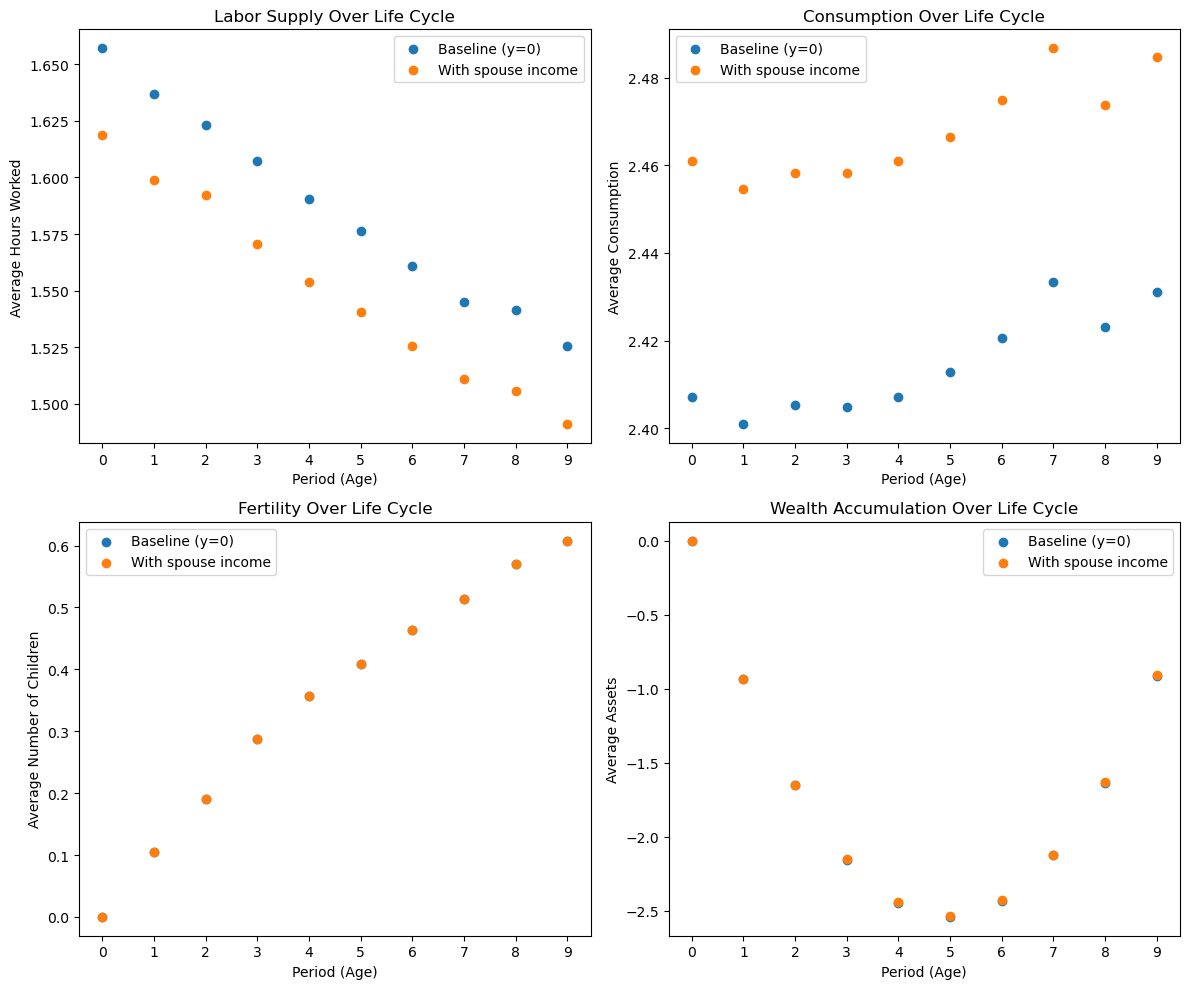
\includegraphics[width=0.5\linewidth]{Billeder/Lifecycle profiles_Q2_Ass1.png}
    \caption{Life-cycle profiles of labour supply, consumption, fertility, and assets in the baseline model and in the model with spouse income.}
    \label{fig:q2_profiles}
\end{figure}